\section{Exercises}

%_________________
\subsection{Defining probability}

% 1

\eoce{\qt{True or false} Determine if the statements below are true or false, and explain your reasoning.
\begin{parts}
\item If a fair coin is tossed many times and the last eight tosses are all heads, then the chance that the next toss will be heads is somewhat less than 50\%.
\item Drawing a face card (jack, queen, or king) and drawing a red card from a full deck of playing cards are mutually exclusive events.
\item Drawing a face card and drawing an ace from a full deck of playing cards are mutually exclusive events.
\end{parts}
}{}

% 2

\eoce{\qt{Roulette wheel\label{roulette_wheel}} The game of roulette involves spinning a wheel with 38 slots: 18 red, 18 black, and 2 green. A ball is spun onto the wheel and will eventually land in a slot, where each slot has an equal chance of capturing the ball. \footfullcite{rouletteWheelPic}

\noindent\begin{minipage}[c]{0.725\textwidth}
\begin{parts}
\item You watch a roulette wheel spin 3 consecutive times and the ball lands on a red slot each time. What is the probability that the ball will land on a red slot on the next spin?
\item You watch a roulette wheel spin 300 consecutive times and the ball lands on a red slot each time. What is the probability that the ball will land on a red slot on the next spin?
\item Are you equally confident of your answers to parts~(a) and~(b)? Why or why not?
\end{parts}
\end{minipage}
\begin{minipage}[c]{0.025\textwidth}
\end{minipage}
\begin{minipage}[c]{0.25\textwidth}
\hfill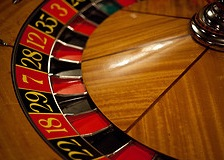
\includegraphics[width = 0.94\textwidth]{02/figures/eoce/images/roulette_wheel}
\end{minipage}
}{}


% 3

\eoce{\qt{Four games, one winner} Below are four versions of the same game. Your archnemisis gets to pick the version of the game, and then you get to choose how many times to flip a coin: 10 times or 100 times. Identify how many coin flips you should choose for each version of the game. Explain your reasoning.
\begin{parts}
\item If the proportion of heads is larger than 0.60, you win \$1.
\item If the proportion of heads is larger than 0.40, you win \$1.
\item If the proportion of heads is between 0.40 and 0.60, you win \$1.
\item If the proportion of heads is smaller than 0.30, you win \$1.
\end{parts}
}{}

% 4

\eoce{\qt{Backgammon} Backgammon is a board game for two players in which the playing pieces are moved according to the roll of two dice. Players win by removing all of their pieces from the board, so it is usually good to roll high numbers. You are playing backgammon with a friend and you roll two 6s in your first roll and two 6s in your second roll. Your friend rolls two 3s in his first roll and again in his second row. Your friend claims that you are cheating, because rolling double 6s twice in a row is very unlikely. Using probability, show that your rolls were just as likely as his.
}{}

% 5

\eoce{\qt{Coin flips} If you flip a fair coin 10 times, what is the probability of \vspace{-3mm}
\begin{multicols}{3}
\begin{parts}
\item getting all tails? 
\item getting all heads? 
\item getting at least one tails? 
\end{parts}
\end{multicols}
}{}

% 6

\eoce{\qt{Dice rolls} If you roll a pair of fair dice, what is the probability of \textB{\vspace{-3mm}}
\begin{multicols}{3}
\begin{parts}
\item getting a sum of 1?
\item getting a sum of 5?
\item getting a sum of 12?
\end{parts}
\end{multicols} 
}{}

% 7
\textB{\pagebreak}

\eoce{\qt{Swing voters\label{indepSwing}} A 2012 Pew Research survey asked 2,373 randomly sampled registered voters their political affiliation (Republican, Democrat, or Independent) and whether or not they identify as swing voters. 35\% of respondents identified as Independent, 23\% identified as swing voters, and 11\% identified as both.\footfullcite{indepSwing}
\begin{parts}
\item Are being Independent and being a swing voter disjoint, i.e. mutually exclusive?
\item Draw a Venn diagram summarizing the variables and their associated probabilities.
\item What percent of voters are Independent but not swing voters?
\item What percent of voters are Independent or swing voters?
\item What percent of voters are neither Independent nor swing voters?
\item Is the event that someone is a swing voter independent of the event that someone is a political Independent?
\end{parts}
}{}

% 8

\eoce{\qt{Poverty and language\label{poorLang}} The American Community Survey is an ongoing survey that provides data every year to give communities the current information they need to plan investments and services. The 2010 American Community Survey estimates that 14.6\% of Americans live below the poverty line, 20.7\% speak a language other that English at home, and 4.2\% fall into both categories. \footfullcite{poorLang}
\begin{parts}
\item Are living below the poverty line and speaking a language other than English at home disjoint?
\item Draw a Venn diagram summarizing the variables and their associated probabilities.
\item What percent of Americans live below the poverty line and only speak English at home?
\item What percent of Americans live below the poverty line or speak a language other than English at home?
\item What percent of Americans live above the poverty line and only speak English at home? 
\item Is the event that someone lives below the poverty line independent of the event that the person speaks a language other than English at home?
\end{parts}
}{}

% 9

\eoce{\qt{Disjoint vs. independent} In parts~(a) and~(b), identify whether the events are disjoint, independent, or neither (events cannot be both disjoint and independent).
\begin{parts}
\item You and a randomly selected student from your class both earn A's in this course. 
\item You and your class study partner both earn A's in this course.
\item If two events can occur at the same time, must they be dependent?
\end{parts}
}{}

% 10

\eoce{\qt{Guessing on an exam} In a multiple choice exam, there are 5 questions and 4 choices for each question (a, b, c, d). Nancy has not studied for the exam at all and decides to randomly guess the answers. What is the probability that:
\begin{parts}
\item the first question she gets right is the $5^{th}$ question?
\item she gets all of the questions right?
\item she gets at least one question right?
\end{parts}
}{}

% 11
\textB{\pagebreak}

\eoce{\qt{Educational attainment of couples} The table below shows the distribution of education level attained by US residents by gender based on data collected during the 2010 American Community Survey.\footfullcite{eduSex}
\begin{center}
\begin{tabular}{l p{7cm} c c }
&						& \multicolumn{2}{c}{\textit{Gender}} \\
\cline{3-4}
&												& Male	& Female \\
\cline{2-4}
& Less than 9th grade								&0.06	&0.06	 \\
& 9th to 12th grade, no diploma						&0.10	&0.09	 \\
\textit{Highest} & High school graduate, GED, or alternative	&0.30	&0.20	 \\
\textit{education} & Some college, no degree				&0.22	&0.24	 \\ 
\textit{attained} & Associate's degree					&0.06	&0.08	 \\
& Bachelor's degree									&0.16	&0.17	 \\
& Graduate or professional degree						&0.09	&0.09	 \\
\cline{2-4}
& Total											& 1.00	& 1.00
\end{tabular}
\end{center}
\begin{parts}
\item What is the probability that a randomly chosen man has at least a Bachelor's degree?
\item What is the probability that a randomly chosen woman has at least a Bachelor's degree?
\item What is the probability that a man and a woman getting married both have at least a Bachelor's degree? Note any assumptions you must make to answer this question.
\item If you made an assumption in part~(c), do you think it was reasonable? If you didn't make an assumption, double check your earlier answer and then return to this part.
\end{parts}
}{}

% 12

\eoce{\qt{School absences\label{elementarySchoolSick}} Data collected at elementary schools in DeKalb County, GA suggest that each year roughly 25\% of students miss exactly one day of school, 15\% miss 2 days, and 28\% miss 3 or more days due to sickness. \footfullcite{Mizan:2011}
\begin{parts}
\item What is the probability that a student chosen at random doesn't miss any days of school due to sickness this year?
\item What is the probability that a student chosen at random misses no more than one day?
\item What is the probability that a student chosen at random misses at least one day?
\item If a parent has two kids at a DeKalb County elementary school, what is the probability that neither kid will miss any school? Note any assumption you must make to answer this question.
\item If a parent has two kids at a DeKalb County elementary school, what is the probability that that both kids will miss some school, i.e. at least one day? Note any assumption you make.
\item If you made an assumption in part~(d) or~(e), do you think it was reasonable? If you didn't make any assumptions, double check your earlier answers.
\end{parts}
}{}

% 13

\eoce{\qt{Grade distributions} Each row in the table below is a proposed grade distribution for a class. Identify each as a valid or invalid probability distribution, and explain your reasoning.
\begin{center}
\begin{tabular}{l  ccccc} 
	& \multicolumn{5}{c}{\textit{Grades}} \\
\cline{2-6}
	& A		& B 		& C 		& D		& F  \\
\cline{2-6}
(a) 	& 0.3 	& 0.3 	& 0.3 	& 0.2 	& 0.1\\
(b) 	& 0	 	& 0	 	& 1		& 0		& 0 \\
(c) 	& 0.3 	& 0.3 	& 0.3		& 0		& 0 \\
(d) 	& 0.3 	& 0.5 	& 0.2		& 0.1		& -0.1 \\
(e) 	& 0.2 	& 0.4 	& 0.2		& 0.1		& 0.1 \\
(f) 	& 0	 	& -0.1 	& 1.1		& 0		& 0 \\
\end{tabular}
\end{center}
}{}

% 14
\textB{\pagebreak}

\eoce{\qt{Weight and health coverage, Part I\label{healthCovBMI}} The Behavioral Risk Factor Surveillance System (BRFSS) is an annual telephone survey designed to identify risk factors in the adult population and report emerging health trends. The following table summarizes two variables for the respondents: weight status using body mass index (BMI) and health coverage, which describes whether each respondent had health insurance. \footfullcite{data:BRFSS2010}

\begin{center}
\begin{tabular}{ll  ccc  c} 
			&	\multicolumn{1}{c}{}	& \multicolumn{3}{c}{\textit{Weight Status}} & \\ 
\cline{3-5}
			&		& Neither overweight 	& Overweight 	& Obese	&   \\
			&		& nor obese (BMI $<$ 25)&(25 $\le$ BMI $<$ 30) & (BMI $\ge$ 30) & Total \\
\cline{2-6}
\textit{Health}	&Yes 	& 134,801 	& 141,699 	& 107,301 		& 383,801\\
\textit{Coverage}&No 	& 15,098 		& 15,327 		& 14,412			& 44,837 \\
\cline{2-6}
			&Total	& 149,899		&157,026		& 121,713			& 428,638
\end{tabular}
\end{center}

\begin{parts}
\item If we draw one individual at random, what is the probability that the respondent is overweight and doesn't have health coverage?
\item If we draw one individual at random, what is the probability that the respondent is overweight or doesn't have health coverage?
\end{parts}
}{}


%_________________
\subsection{Conditional probability}

% 15

\eoce{\qt{Joint and conditional probabilities} P(A) = 0.3, P(B) = 0.7
\begin{parts}
\item Can you compute P(A and B) if you only know P(A) and P(B)?
\item Assuming that events A and B arise from independent random processes,
\begin{subparts}
\item what is P(A and B)?
\item what is P(A or B)?
\item what is P(A$|$B)?
\end{subparts}
\item If we are given that P(A and B) = 0.1, are the random variables giving rise to events A and B independent?
\item If we are given that P(A and B) = 0.1, what is P(A$|$B)?
\end{parts}
}{}

% 16

\eoce{\qt{PB \& J} Suppose 80\% of people like peanut butter, 89\% like jelly, and 78\% like both. Given that a randomly sampled person likes peanut butter, what's the probability that he also likes jelly?
}{}

% 17

\eoce{\qt{Global warming} A 2010 Pew Research poll asked 1,306 Americans ``From what you've read and heard, is there solid evidence that the average temperature on earth has been getting warmer over the past few decades, or not?". The table below shows the distribution of responses by party and ideology, where the counts have been replaced with relative frequencies.\footfullcite{globalWarming}
\begin{center}
\begin{tabular}{ll  ccc c} 
							&			& \multicolumn{3}{c}{\textit{Response}} \\
\cline{3-5}
							&			& Earth is 		& Not 		& Don't Know	&	\\
							&			& warming	& warming 	& Refuse		& Total\\
\cline{2-6}
				& Conservative Republican	& 0.11	 	& 0.20		& 0.02 		& 0.33 	\\
\textit{Party and}	& Mod/Lib Republican		& 0.06	 	& 0.06 	 	& 0.01		& 0.13 \\
\textit{Ideology}		& Mod/Cons Democrat		& 0.25	 	& 0.07 	 	& 0.02 		& 0.34 \\
				& Liberal Democrat			& 0.18	 	& 0.01 	 	& 0.01 		& 0.20\\
\cline{2-6}
							&Total		& 0.60		& 0.34		& 0.06		& 1.00
\end{tabular}
\end{center}
\begin{parts}
\item What is the probability that a randomly chosen respondent believes the earth is warming or is a liberal Democrat?
\item What is the probability that a randomly chosen respondent believes the earth is warming given that he is a liberal Democrat?
\item What is the probability that a randomly chosen respondent believes the earth is warming given that he is a conservative Republican?
\item Does it appear that whether or not a respondent believes the earth is warming is independent of their party and ideology? Explain your reasoning.
\item What is the probability that a randomly chosen respondent is a moderate/liberal Republican given that he does not believe that the earth is warming? 
\end{parts}
}{}

% 18

\eoce{\qt{Weight and health coverage, Part II} Exercise~\ref{healthCovBMI} introduced a contingency table summarizing the relationship between weight status, which is determined based on body mass index (BMI), and health coverage for a sample of 428,638 Americans. In the table below, the counts have been replaced by relative frequencies (probability estimates).

\begin{center}
\begin{tabular}{ll  ccc  c} 
			&	\multicolumn{1}{c}{}	& \multicolumn{3}{c}{\textit{Weight Status}} & \\ 
\cline{3-5}
			&		& Neither overweight 	& Overweight 	& Obese	&   \\
			&		& nor obese (BMI $<$ 25)&(25 $\le$ BMI $<$ 30) & (BMI $\ge$ 30) & Total \\
\cline{2-6}
\textit{Health}	&Yes 	& 0.3145	 	& 0.3306	 	& 0.2503	 		& 0.8954\\
\textit{Coverage}&No 	& 0.0352 		& 0.0358 		& 0.0336			& 0.1046 \\
\cline{2-6}
			&Total	& 0.3497		&0.3664		& 0.2839			& 1.0000
\end{tabular}
\end{center}

\begin{parts}
\item What is the probability that a randomly chosen individual is obese?
\item What is the probability that a randomly chosen individual is obese given that he has health coverage?
\item What is the probability that a randomly chosen individual is obese given that he doesn't have health coverage?
\item Do being overweight and having health coverage appear to be independent?
\end{parts}
}{}

% 19

\eoce{\qt{Burger preferences} A 2010 SurveyUSA poll asked 500 Los Angeles residents, ``What is the best hamburger place in Southern California? Five Guys Burgers? In-N-Out Burger? Fat Burger? Tommy's Hamburgers? Umami Burger? Or somewhere else?'' The distribution of responses by gender is shown below. \footfullcite{burgers}
\begin{center}
\begin{tabular}{l p{4cm} r r r }
&						& \multicolumn{2}{c}{\textit{Gender}} \\
\cline{3-4}
&								& Male	& Female 	& Total\\
\cline{2-5}
& Five Guys Burgers					&5		&6	 	& 11	\\
& In-N-Out Burger					&162	&181	& 343 \\
\textit{Best} & Fat Burger				&10		&12	 	& 22 \\
\textit{hamburger} & Tommy's Hamburgers	&27		&27	 	& 54	\\ 
\textit{place} & Umami Burger			&5		&1	 	& 6 \\
& Other							&26		&20	 	& 46 \\
& Not Sure						&13		&5	 	& 18 \\
\cline{2-5}
&Total							&248	&252	& 500
\end{tabular}
\end{center}
\begin{parts}
\item What is the probability that a randomly chosen male likes In-N-Out the best?
\item What is the probability that a randomly chosen female likes In-N-Out the best?
\item What is the probability that a man and a woman who are dating both like In-N-Out the best? Note any assumption you make and evaluate whether you think that assumption is reasonable.
\item What is the probability that a randomly chosen person likes Umami best or that person is female?
\end{parts}
}{}

% 20

\eoce{\qt{Assortative mating} Assortative mating is a nonrandom mating pattern where individuals with similar genotypes and/or phenotypes mate with one another more frequently than what would be expected under a random mating pattern. Researchers studying this topic collected data on eye colors of  204 Scandinavian men and their female partners. The table below summarizes the results. For simplicity, we only include heterosexual relationships in this exercise. \footfullcite{Laeng:2007}
\begin{center}
\begin{tabular}{ll  ccc c} 
							&			& \multicolumn{3}{c}{\textit{Partner (female)}} \\
\cline{3-5}
							&			& Blue 	& Brown	& Green 	& Total	\\
\cline{2-6}
							&Blue 		& 78	 	& 23		& 13		& 114 	\\
\multirow{2}{*}{\textit{Self (male)}}	&Brown		& 19	 	& 23 	 	& 12		& 54 \\
							&Green		& 11	 	& 9 	 	& 16		& 36 \\
\cline{2-6}	
							&Total		& 108	& 55		& 41		& 204
\end{tabular}
\end{center}
\begin{parts}
\item What is the probability that a randomly chosen male respondent or his partner has blue eyes?
\item What is the probability that a randomly chosen male respondent with blue eyes has a partner with blue eyes? 
\item What is the probability that a randomly chosen male respondent with brown eyes has a partner with blue eyes? What about the probability of a randomly chosen male respondent with green eyes having a partner with blue eyes?
\item Does it appear that the eye colors of male respondents and their partners are independent? Explain your reasoning.
\end{parts}
}{}

% 21

\eoce{\qt{Drawing box plots\label{constructingBoxPlots}} After an introductory statistics course, 80\% of students can successfully construct box plots. Of those who can construct box plots, 86\% passed, while only 65\% of those students who could not construct box plots passed.
\begin{parts}
\item Construct a tree diagram of this scenario.
\item Calculate the probability that a student is able to construct a box plot if it is known that he passed.
\end{parts}
}{}

% 22

\eoce{\qt{Predisposition for thrombosis} A genetic test is used to determine if people have a predisposition for \textit{thrombosis}, which is the formation of a blood clot inside a blood vessel that obstructs the flow of blood through the circulatory system. It is believed that 3\% of people actually have this predisposition. The genetic test is 99\% accurate if a person actually has the predisposition, meaning that the probability of a positive test result when a person actually has the predisposition is 0.99. The test is 98\% accurate if a person does not have the predisposition. What is the probability that a randomly selected person who tests positive for the predisposition by the test actually has the predisposition?
}{}

% 23

\eoce{\qt{HIV in Swaziland} Swaziland has the highest HIV prevalence in the world: 25.9\% of this country's population is infected with HIV.\footfullcite{ciaFactBookHIV:2012} The ELISA test is one of the first and most accurate tests for HIV. For those who carry HIV, the ELISA test is 99.7\% accurate. For those who do not carry HIV, the test is 92.6\% accurate. If an individual from Swaziland has tested positive, what is the probability that he carries HIV?
}{}

% 24

\eoce{\qt{Exit poll} Edison Research gathered exit poll results from several sources for the Wisconsin recall election of Scott Walker. They found that 53\% of the respondents voted in favor of Scott Walker. Additionally, they estimated that of those who did vote in favor for Scott Walker, 37\% had a college degree, while 44\% of those who voted against Scott Walker had a college degree. Suppose we randomly sampled a person who participated in the exit poll and found that he had a college degree. What is the probability that he voted in favor of Scott Walker?\footfullcite{data:scott}
}{}


%_________________
\subsection{Sampling from a small population}

% 27

\eoce{\qt{Urns and marbles, Part I\label{urnWithMarbles}} Imagine you have an urn containing 5 red, 3 blue, and 2 orange marbles in it. 
\begin{parts}
\item What is the probability that the first marble you draw is blue?
\item Suppose you drew a blue marble in the first draw. If drawing with replacement, what is the probability of drawing a blue marble in the second draw?
\item Suppose you instead drew an orange marble in the first draw. If drawing with replacement, what is the probability of drawing a blue marble in the second draw?
\item If drawing with replacement, what is the probability of drawing two blue marbles in a row?
\item When drawing with replacement, are the draws independent? Explain.
\end{parts}
}{}

% 28

\eoce{\qt{Socks in a drawer} In your sock drawer you have 4 blue, 5 gray, and 3 black socks. Half asleep one morning you grab 2 socks at random and put them on. Find the probability you end up wearing
\begin{parts}
\item 2 blue socks
\item no gray socks
\item at least 1 black sock
\item a green sock
\item matching socks
\end{parts}
}{}


% 29

\eoce{\qt{Urns and marbles, Part II} Imagine you have an urn containing 5 red, 3 blue, and 2 orange marbles.
\begin{parts}
\item Suppose you draw a marble and it is blue. If drawing without replacement, what is the probability the next is also blue?
\item Suppose you draw a marble and it is orange, and then you draw a second marble without replacement. What is the probability this second marble is blue?
\item If drawing without replacement, what is the probability of drawing two blue marbles in a row?
\item When drawing without replacement, are the draws independent? Explain.
\end{parts}
}{}

% 30
\textB{\pagebreak}

\eoce{\qt{Books on a bookshelf} The table below shows the distribution of books on a bookcase based on whether they are nonfiction or fiction and hardcover or paperback. \vspace{-2.5mm}
\begin{center}
\begin{tabular}{ll  cc c} 
							&			& \multicolumn{2}{c}{\textit{Format}} \\
\cline{3-4}
							&			& Hardcover 	& Paperback 	& Total	\\
\cline{2-5}
\multirow{2}{*}{\textit{Type}}		&Fiction 		& 13	 		& 59			& 72 	\\
							&Nonfiction	& 15	 		& 8 	 		& 23 \\
\cline{2-5}	
							&Total		& 28			& 67			& 95 \\
\cline{2-5}
\end{tabular}
\end{center} \vspace{-2.5mm}
\begin{parts}
\item Find the probability of drawing a hardcover book first then a paperback fiction book second when drawing without replacement.
\item Determine the probability of drawing a fiction book first and then a hardcover book second, when drawing without replacement.
\item Calculate the probability of the scenario in part~(b), except this time complete the calculations under the scenario where the first book is placed back on the bookcase before randomly drawing the second book.
\item The final answers to parts~(b) and~(c) are very similar. Explain why this is the case.
\end{parts}
}{}

% 31

\eoce{\qt{Student outfits} In a classroom with 24 students, 7 students are wearing jeans, 4 are wearing shorts, 8 are wearing skirts, and the rest are wearing leggings. If we randomly select 3 students without replacement, what is the probability that one of the selected students is wearing leggings and the other two are wearing jeans? Note that these are mutually exclusive clothing options.
}{}

% 32

\eoce{\qt{The birthday problem} Suppose we pick three people at random. For each of the following questions, ignore the special case where someone might be born on February 29th, and assume that births are evenly distributed throughout the year.
\begin{parts}
\item What is the probability that the first two people share a birthday? 
\item What is the probability that at least two people share a birthday?
\end{parts}
}{}


%_________________
\subsection{Random variables}

% 33

\eoce{\qt{College smokers} At a university, 13\% of students smoke.
\begin{parts}
\item Calculate the expected number of smokers in a random sample of 100 students from this university.
\item The university gym opens at 9am on Saturday mornings. One Saturday morning at 8:55am there are 27 students outside the gym waiting for it to open. Should you use the same approach from part (a) to calculate the expected number of smokers among these 27 students?
\end{parts}
}{}

% 34

\eoce{\qt{Card game} Consider the following card game with a well-shuffled deck of cards. If you draw a red card, you win nothing. If you get a spade, you win \$5. For any club, you win \$10 plus an extra \$20 for the ace of clubs.
\begin{parts}
\item Create a probability model for the amount you win at this game. Also, find the expected winnings for a single game and the standard deviation of the winnings.
\item What is the maximum amount you would be willing to pay to play this game? Explain.
\end{parts}
}{}

% 35

\eoce{\qt{Another card game} In a new card game, you start with a well-shuffled full deck and draw 3 cards without replacement. If you draw 3 hearts, you win \$50. If you draw 3 black cards, you win \$25. For any other draws, you win nothing.
\begin{parts}
\item Create a probability model for the amount you win at this game, and find the expected winnings. Also compute the standard deviation of this distribution.
\item If the game costs \$5 to play, what would be the expected value and standard deviation of the net profit (or loss)? \textit{(Hint: profit = winnings $-$ cost; $X-5$)}
\item If the game costs \$5 to play, should you play this game? Explain.
\end{parts}
}{}

% 36

\eoce{\qtq{Is it worth it} Andy is always looking for ways to make money fast. Lately, he has been trying to make money by gambling. Here is the game he is considering playing: The game costs \$2 to play. He draws a card from a deck. If he gets a number card (2-10), he wins nothing. For any face card (jack, queen or king), he wins \$3. For any ace, he wins \$5, and he wins an \textit{extra} \$20 if he draws the ace of clubs.
\begin{parts}
\item Create a probability model and find Andy's expected profit per game.
\item Would you recommend this game to Andy as a good way to make money? Explain.
\end{parts}
}{}

% 37

\eoce{\qt{Portfolio return} A portfolio's value increases by 18\% during a financial boom and by 9\% during normal times. It decreases by 12\% during a recession. What is the expected return on this portfolio if each scenario is equally likely?
}{}

% 38

\eoce{\qt{A game of roulette, Part I\label{roulette}} The game of roulette involves spinning a wheel with 38 slots: 18 red, 18 black, and 2 green. A ball is spun onto the wheel and will eventually land in a slot, where each slot has an equal chance of capturing the ball. Gamblers can place bets on red or black. If the ball lands on their color, they double their money. If it lands on another color, they lose their money. Suppose you bet \$1 on red. What's the expected value and standard deviation of your winnings?
}{}

% 39

\eoce{\qt{A game of roulette, Part II} Exercise~\ref{roulette} describes winnings on a game of roulette.
\begin{parts}
\item Suppose you play roulette and bet \$3 on a single round. What is the expected value and standard deviation of your total winnings?
\item Suppose you bet \$1 in three different rounds. What is the expected value and standard deviation of your total winnings?
\item How do your answers to parts (a) and (b) compare? What does this say about the riskiness of the two games?
\end{parts}
}{}

% 40

\eoce{\qt{Baggage fees\label{americanAir}} An airline charges the following baggage fees: \$25 for the first bag and \$35 for the second. Suppose 54\% of passengers have no checked luggage, 34\% have one piece of checked luggage and 12\% have two pieces. We suppose a negligible portion of people check more than two bags.
\begin{parts}
\item Build a probability model, compute the average revenue per passenger, and compute the corresponding standard deviation.
\item About how much revenue should the airline expect for a flight of 120 passengers? With what standard deviation? Note any assumptions you make and if you think they are justified.
\end{parts}
}{}

% 41

\eoce{\qt{Dodgers vs. Padres} You and your friend decide to bet on the Major League Baseball game happening one evening between the Los Angeles Dodgers and the San Diego Padres. Suppose current statistics indicate that the Dodgers have a 0.46 probability of winning this game against the Padres. If your friend bets you \$5 that the Dodgers will win, how much would you need to bet on the Padres to make this a fair game?
}{}

% 42

\eoce{\qt{Selling on Ebay} Marcie has been tracking the following two items on Ebay:
\begin{itemize}
\item A textbook that sells for an average of \$110 with a standard deviation of \$4.
\item Mario Kart for the Nintendo Wii, which sells for an average of \$38 with a standard deviation of \$5.
\end{itemize}
\begin{parts}
\item Marcie wants to sell the video game and buy the textbook. How much net money (profits - losses) would she expect to make or spend? Also compute the standard deviation of how much she would make or spend.
\item Lucy is selling the textbook on Ebay for a friend, and her friend is giving her a 10\% commission (Lucy keeps 10\% of the revenue). How much money should she expect to make? With what standard deviation?
\end{parts}
}{}

% 43

\eoce{\qt{Cost of breakfast} Sally gets a cup of coffee and a muffin every day for breakfast from one of the many coffee shops in her neighborhood. She picks a coffee shop each morning at random and independently of previous days. The average price of a cup of coffee is \$1.40 with a standard deviation of 30\textcent (\$0.30), the average price of a muffin is \$2.50 with a standard deviation of 15\textcent, and the two prices are independent of each other.
\begin{parts}
\item What is the mean and standard deviation of the amount she spends on breakfast daily?
\item What is the mean and standard deviation of the amount she spends on breakfast weekly (7~days)?
\end{parts}
}{}

% 44

\eoce{\qt{Ice cream} Ice cream usually comes in 1.5 quart boxes (48 fluid ounces), and ice cream scoops hold about 2 ounces. However, there is some variability in the amount of ice cream in a box as well as the amount of ice cream scooped out. We represent the amount of ice cream in the box as $X$ and the amount scooped out as $Y$. Suppose these random variables have the following means, standard deviations, and variances:
\begin{center}
\begin{tabular}{l ccc}
\hline
	& mean & SD & variance \\
\hline
$X$	& 48	   & 1		& 1		\\
$Y$ & 2	   & 0.25	& 0.0625	\\
\hline
\end{tabular}
\end{center}
\begin{parts}
\item An entire box of ice cream, plus 3 scoops from a second box is served at a party. How much ice cream do you expect to have been served at this party? What is the standard deviation of the amount of ice cream served?
\item How much ice cream would you expect to be left in the box after scooping out one scoop of ice cream? That is, find the expected value of $X-Y$. What is the standard deviation of the amount left in the box?
\item Using the context of this exercise, explain why we add variances when we subtract one random variable from another.
\end{parts}
}{}


%_________________
\subsection{Continuous distributions}

% 45

\eoce{\qt{Cat weights\label{catsBodyWeights}} The histogram shown \textB{below} represents the weights (in kg) of 47 female and 97 male cats. \footfullcite{cats} \\
\begin{minipage}[c]{0.4\textwidth}
\begin{parts}
\item What fraction of these cats weigh less than 2.5 kg?
\item What fraction of these cats weigh between 2.5 and 2.75 kg?
\item What fraction of these cats weigh between 2.75 and 3.5 kg?
\end{parts} \vspace{27mm}
\end{minipage}
\begin{minipage}[c]{0.05\textwidth}
$\:$ 
\end{minipage}
\begin{minipage}[c]{0.55\textwidth}
\begin{center}
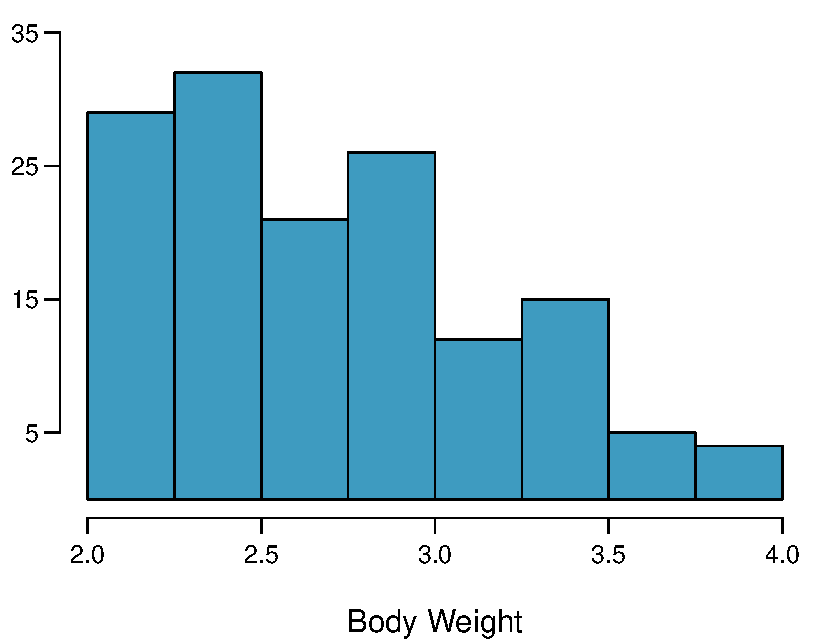
\includegraphics[width=\textwidth]{02/figures/eoce/cats/cats_bodyWeight}
\end{center}
\end{minipage}
}{}

% 46
\textB{\pagebreak}

\eoce{\qt{Income and gender} The relative frequency table below displays the distribution of annual total personal income (in 2009 inflation-adjusted dollars) for a representative sample of 96,420,486 Americans. These data come from the American Community Survey for 2005-2009. This sample is comprised of 59\% males and 41\% females. \footfullcite{acsIncome2005-2009} \\

\noindent\begin{minipage}[c]{0.60\textwidth}
\begin{parts}
\item Describe the distribution of total personal income.
\item What is the probability that a randomly chosen US resident makes less than \$50,000 per year?
\item What is the probability that a randomly chosen US resident makes less than \$50,000 per year and is female? Note any assumptions you make.
\item The same data source indicates that 71.8\% of females make less than \$50,000 per year. Use this value to determine whether or not the assumption you made in part (c) is valid.
\end{parts} 
\end{minipage}
\begin{minipage}[c]{0.4\textwidth}
{\small
\begin{center}
\begin{tabular}{lr}
  \hline
\multicolumn{1}{c}{\textit{Income}}		& \multicolumn{1}{c}{\textit{Total}} \\
  \hline
\$1 to \$9,999 or loss	&2.2\%	\\
\$10,000 to \$14,999		&4.7\%	\\
\$15,000 to \$24,999		&15.8\%	\\
\$25,000 to \$34,999		&18.3\%	\\
\$35,000 to \$49,999		&21.2\%	\\
\$50,000 to \$64,999		&13.9\%	\\
\$65,000 to \$74,999		&5.8\%	\\
\$75,000 to \$99,999		&8.4\%	\\
\$100,000 or more		&9.7\%	\\
   \hline
\end{tabular}
\end{center}
}
\end{minipage} \\
}{}

